\section{Imitation Learning}
Defining complex tasks, such as driving a car, is often very challenging. 
In reinforcement learning, agents typically learn by receiving rewards that
signal how good their actions are. However, in many real-world scenarios, especially
those involving human skills like driving, designing an explicit reward function is difficult
and often impractical. Humans, on the other hand, are naturally good at demonstrating how to 
perform such tasks.\newline 
The idea behind imitation learning is to infer the underlying policy by observing an expert, 
without access to a reward function. 
%In this approach, we are given a set of trajectories, which were generated by an expert: $\tau_n = ((s_1,a_1),\dots,(s_{T_n},a_{T_n}))$ Our task is to learn a policy without knowing the reward. 
Therefore, the setting for imitation learning is as follows:
\begin{itemize}
    \item set of trajectories $D = \{\tau_1,\dots,\tau_N\}$
    \item state action pairs  $\tau_n = ((s_1,a_1),\dots,(s_{T_n},a_{T_n}))$ generated by the expert
    \item transition/ system dynamics $P(s'|s,a)$
    \item underlying/observation policy $\pi_{\text{dem}}(a_t|s_t)$
    \item agent policy $\pi_\theta(a_t|s_t)$
    %\item state-action occupancy of policy $\pi: \rho_\pi(s,a)= \pi(a|s)\underset{t}{\sum}P(s_t=s|\pi)$
    %\item state  occupancy of policy $\rho_\pi(a) = \underset{a}{\sum}\rho_\pi(s,a)$
\end{itemize}

\subsection{Behavioural Cloning}
One approach is to reduce the problem to a supervised learning task, where we aim to learn 
the mapping from states to actions. Specifically we want to minimizes the Kullback–Leibler between the expert policy  
 $\pi_\text{dem}$ and learned policy $\pi_\theta$ . The objective can be written as:
\begin{align*}
    \pi_\theta^* &= \argmin\limits_\theta \underset{D\sim s}{\mathbb{E}}\left[D_{\text{KL}}(\pi_{\text{dem}}(a|s)|| \pi_\theta(a|s))\right] \\
    %&=  \argmin\limits_\theta \underset{D\sim s}{\mathbb{E}}\left[\mathbb{E}_{a\sim \pi_\text{dem}}\left[\log{\frac{\pi_\text{dem}(a|s)}{\pi_\theta(a|s)}}\right]\right] \\
    %&=  \argmin\limits_\theta \underset{D\sim s}{\mathbb{E}}\left[\mathbb{E}_{a\sim \pi_\text{dem}}\left[\log{\pi_\text{dem}(a|s)}-\log{\pi_\theta(a|s)}\right]\right] \\
    %  &=  \argmin\limits_\theta \underset{D\sim s}{\mathbb{E}}[\underbrace{\mathbb{E}_{a\sim \pi_\text{dem}}[\log{\pi_\text{dem}(a|s)}]}_{\text{const: doesn't depend on $\theta$}}-\mathbb{E}_{a\sim \pi_\text{dem}}[\log{\pi_\theta(a|s)}]] \\
    &= \argmin\limits_\theta \underset{D\sim(s,a)}{\mathbb{E}}[-\log{\pi_\theta(a|s)}]+C
\end{align*}
Thus, the problem reduces to maximum likelihood estimation (MLE). However, there are a few notable issues with this approach.

\subsubsection{Distributional Shift}
The primary problem in respect to behaviour cloning is the distributional shift. 
Specifically, the network is trained only on the dataset $D$ from the expert, but 
at test time, it receives its own potentially incorrect predictions as inputs (due to 
stochastic policy, stochastic system dynamics etc.). 
This leads to the agent entering regions of the state space it hasn't learned from, due to small 
compounding errors. As a result, for states it has never observed, the agent doesn't 
know how to behave, leading to poor policies. The core issue is that the distribution of inputs 
the model encounters at test time differs from the distribution it was trained on (distributional shift).\newline   
A solution to this problem is an algorithm called \textbf{DAgger} (Dataset Aggregation). DAgger starts similarly to standard behavior 
cloning: we train a policy using expert demonstrations. The key difference is that, after we deployed it in the environment to collect new 
data to train on we query the expert to label the correct actions that should have been taken in each state. These corrected state-action 
pairs are added to the dataset, and the policy is retrained on the aggregated data. This process is repeated iteratively, gradually improving 
the policy and reducing distributional shift.
\begin{algorithm}[H]
  %\large
    \caption{DAgger}\label{algo:dagger}
    \begin{algorithmic}
    \FOR{$k=1\dots n$}
    \STATE train policy from data $D \rightarrow \pi_{\theta}$
    \STATE run policy to collect new data $\pi_{\theta}\rightarrow D_{\theta}$
    \STATE where necessary ask expert for advise $D_{\theta} \rightarrow D_{\theta} \bigoplus a_{\text{expert}}$
    \STATE Aggregate Data $D \cup D_{\theta} \rightarrow D$    
    \ENDFOR
    \end{algorithmic}
\end{algorithm}
However, the obvious problem with this approach is that collecting additional training data is very expensive. 
Beyond that, there are two other challenges that make it difficult to learn the optimal policy.

\paragraph{Markovian System}
Another problem preventing us from learning good policies is the assumption that the 
system is Markovian. In many cases, the states we've visited before have a significant 
impact on our decision-making at the current time step. This means humans do not act in a 
purely Markovian way. A simple solution to this is to use non-Markovian policies, which we 
could implement with Recurrent Neural Networks (RNNs).

\paragraph{Multimodal Behavoiur}
Yet another problem is multimodal behaviour. Consider the case of flying a drone, where the 
dataset includes a state where the drone must fly around a tree, either to the left or to 
the right. In the dataset, half the time we go left and the other half, we go right. For a 
discrete policy, after training, it might give a 50\% probability of going right or left. 
However, for a continuous policy, regression will average out the decision between going 
left or right, resulting in suboptimal behaviour. One solution to this is to output a 
mixture of Gaussians to account for the multimodal nature of the decision. \newline\newline 
Even with these improvements, the fact remains that expert demonstrations provide an upper 
bound for behavioural cloning. This means that we are only as good as the expert. However, 
if we could understand the intention behind the expert's actions, we might be able to 
develop better policies beyond simply mimicking the expert.

\subsection{Inverse Reinforcement Learning}
In Inverse Reinforcement Learning (IRL), the goal is to infer the reward function from a 
given set of expert demonstrations so that the expert policy is optimal under this reward function,
and then use this reward function to learn a policy. However, there are two main issues with this approach:
\begin{enumerate}
    \item the demonstrations could have been produced by many policies
    \item the are many reward function for which the experts policy is optimal
\end{enumerate}
In the following we are going to look at some methods which try to implement inverse reinforcement learning. 

\subsubsection{Feature Matching}
In the early days, researchers viewed reward functions as being based not directly on 
states and actions, but rather on features $f$ of these states and actions:
$$ r_{\psi}(s,a) = \sum_i \psi_i f_i(s,a) = \psi^T f$$
In reinforcement learning (RL), features are numeric values that represent the state 
(and sometimes the action) of the environment in a form that supports learning. These values
act as inputs to the learning algorithm, helping the agent understand its situation and make decisions.\newline
For example, in the CartPole-v1 environment, the state is described by four features: the cart’s position 
and velocity, the angle of the pole, and the velocity at the pole’s tip. These features capture everything 
the agent needs to know to learn the task. 
%In more complex environments like autonomous driving, features might include the distance to nearby vehicles, relative speed, lane position, road curvature, and traffic light status.\newline
While early RL relied on handcrafted features, modern approaches especially those using deep learning often
learn features directly from raw sensor data. However, not all RL algorithms require explicit features. 
Tabular methods can work with small, discrete state spaces where each state is just an index. But for large
or continuous environments, function approximators like neural networks are used, and these require meaningful
features to work effectively.\newline
The core idea is now that if the right set of features is chosen, we can reproduce expert-like behaviour by ensuring
that the agent matches the expected values of those features. In other words, by aligning the feature expectations 
of the agent with those of the expert we can induce similar behaviour. Formally the objective becomes finding a parameter
vector $\psi$ such that:
$$\mathbb{E}_{\pi^{r_\psi}}[f(s,a)] = \mathbb{E}_{\pi^{*}}[f(s,a)]$$
However, there is still the issue of ambiguity, as different $\psi$ vectors can result in the same expected feature values.

\subsubsection{Max-Entropy Inverse Reinforcement Learning} \label{MaxEntIRL}
Max-Entropy Inverse Reinforcement Learning tries to address the problem of the ambiguity in the reward functions by 
using the principle of maximum entropy. The principle of maximum entropy states that the probability distribution which best 
represents the current state of knowledge about a system is the one with the largest 
entropy. The entropy $H(X)$ is defined as $$H(X) =- \sum_{x\in X} p(x)\log{p(x)}$$ 
The objective is now to maximize the entropy $H(X)$, while ensuring matching the feature count
and ensuring that $p$ is a proper distribution over the expert data set $D$ ($\tau$ are the trajectories)
$$\argmax\limits_\psi - \sum_{\tau\in D} p_\psi(\tau)\log{p_\psi(\tau)} \quad \text{ s.t. } \sum_{\tau} p_\psi(\tau)f(\tau) = \frac{1}{|D|}\sum_{i \in D}f(\tau_i)
\text{ and } \sum_{\tau} p_\psi(\tau) = 1$$
The solution for this constrained problem can be derived using Lagrange multipliers, which leads to the 
solution: 
$$p_\psi(\tau;) \propto \frac{1}{Z(\psi)}\exp{r_{\psi}(\tau)} \text{ with } Z(\psi) = \sum_\tau \exp{r_\psi(\tau)}$$
%$$p(\tau;\omega) = \frac{1}{Z(\omega)}\exp{(\omega^T f(\tau))}$$
%Here $Z(\omega)$  is the normalizing constant, and $\omega$ is the Lagrange multiplier.
%In general, we should not assume a linear reward model. Instead, we could use a neural 
%network to generalize the reward function. In this case, the formula would be updated to: 
%$$p(\tau;\psi) = \frac{1}{Z(\psi)}\exp{r_{\psi}(\tau)}$$. 
Under this principle good behaviour is exponentially more likely. Now, we have a probability distribution over trajectories 
which depends on the reward model, although we do not know the exact model (we do not know the right 
$\psi$). However, we know that the distribution is a normalized exponential distribution. 
This allows us to perform log-maximum likelihood estimation on the parameters of the 
reward model.
\begin{align*}
    \max_\psi \log{\prod_{\tau \in D}p_\psi(\tau)} &= \max_\psi \log{\prod_{\tau \in D}}  \frac{\exp{r_{\psi}(\tau)}}{\sum_{\tau^*} \exp{r_\psi(\tau^*)}} \\
    &=  \max_\psi \sum_{\tau \in D}\left(\log{\exp{r_{\psi}(\tau)}} - \log{\sum_{\tau^*} \exp{r_\psi(\tau^*)}}\right) \\
    &= \max_\psi \sum_{\tau \in D}\log{\exp{r_{\psi}(\tau)}} - |D|\log{\sum_{\tau^*} \exp{r_\psi(\tau^*)}} \\
    &= \max_\psi \sum_{\tau \in D}r_{\psi}(\tau) - |D|\log{\sum_{\tau^*} \exp{r_\psi(\tau^*)}}
\end{align*}
Now taking the derivative of with respect to $\psi$ yields:
\begin{align*}
     \nabla_\psi \left( \sum_{\tau \in D}r_{\psi}(\tau) - |D|\log{\sum_{\tau^*} \exp{r_\psi(\tau^*)}}\right) &=
    \sum_{\tau \in D}   \frac{\diff}{\diff \psi} r_{\psi}(\tau) - |D| \frac{\diff}{\diff \psi}\log{\sum_{\tau^*} \exp{r_\psi(\tau^*)}} \\
    &= \sum_{\tau \in D}  \frac{\diff}{\diff \psi} r_{\psi}(\tau) - |D|
    \underbrace{\frac{1}{\sum_{\tau^*} \exp{r_\psi(\tau^*)}} \sum_{\tau^*} \exp{r_\psi(\tau^*)}}_{p\psi(\tau^*)} 
    \frac{\diff}{\diff \psi} r_\psi(\tau^*) \\
    &= \sum_{\tau \in D}  \frac{\diff}{\diff \psi} r_{\psi}(\tau) - |D| \sum_{\tau^*}p_\psi(\tau^*)  \frac{\diff}{\diff \psi} r_\psi(\tau^*)  \\
    &=  \sum_{s\in \tau \in D}  \frac{\diff}{\diff \psi} r_{\psi}(s) - |D| \sum_{s}p_\psi(s)  \frac{\diff}{\diff \psi} r_\psi(s) 
\end{align*}
The only remaining component is the state occupancies/frequencies $p_\psi(s)$. In the tabular setting, and assuming the dynamics are known, 
we can compute these frequencies using dynamic programming, provided we have already obtained the policy.
\begin{algorithm}[H]
  %\large
    \caption{Computing state frequencies }\label{algo:state_freq}
    \begin{algorithmic}
    \STATE \COMMENT{Goal is to compute $p_\psi(s)$}
    \STATE \COMMENT{$\mu_t(s)$: prob of visiting $s$ at timestep $t$}
    \STATE $\mu_1(s) = p(s_1 = s)$ \COMMENT{initial state distribution of the MDP}
    \FOR{$t=1\dots T$}
    \STATE $\mu_{t+1}(s) = \sum_a \sum_{s'} \mu_t(s')\pi(a|s')P(s|s',a)$
    \ENDFOR
    \STATE $p_\psi(s) = \sum_t \mu_t(s)$
    \end{algorithmic}
\end{algorithm}
The whole max entropy inverse reinforcement learning algorithm is defined as :
\begin{algorithm}[H]
  %\large
    \caption{Max Entropy Inverse Reinforcement Learning  }\label{algo:maxEntIRL}
    \begin{algorithmic}
    \STATE initialize $\psi$ and gather demonstrations $D$
    \FOR{$m=1\dots M $}
    \STATE solve for optimal policy $\pi(a|s)$ w.r.t reward $r_\psi$ (i.e. value iteration)
    \STATE solve for state frequencies $p_\psi(s)$ through algorithm \ref{algo:state_freq} 
    \STATE compute gradient $ \nabla_\psi \mathcal{L} = \sum_{s\in \tau \in D}  \frac{\diff}{\diff \psi} r_{\psi}(s) - |D| \sum_{s}p_\psi(s)  \frac{\diff}{\diff \psi} r_\psi(s) $
    \STATE $\psi \gets \psi + \alpha \nabla_\psi \mathcal{L}$
    \ENDFOR
    \end{algorithmic}
\end{algorithm}
However, there are some caveats to this approach. The first issue is that we need to compute the optimal policy at every iteration. This is 
already somewhat cumbersome but in addition to that we saw in the Dynamic Programming chapter that this process breaks down in high-
dimensional state and action spaces. Also computing the state frequencies and the gradient becomes infeasible or too slow in such high-
dimensional settings. An improved version of this algorithm, which also works in settings where the dynamics are unknown and can be applied 
to large or continuous state and action spaces, can be found in \cite{finn2016guidedcostlearningdeep}.
%\begin{itemize}
%    \item boltzman rational agent required
%    \item only works well in deterministic systems
%\end{itemize}

\subsubsection{Adversarial Methods}
The idea behind adversarial methods is to train a network to produce samples that appear 
to come from the expert demonstration $p^*(x)$. One way to achieve this is through the  
Generative Adversarial Network (GAN) architecture, where we have a generator $p_\theta(x|z)$ that produces 
''fake`` samples, while simultaneously training a discriminator $D_\psi(x) = p_\psi(\text{real data}|x)$ to distinguish between 
data generated by the generator and data from the expert. The objective is for the generator to 
become so good that the discriminator can no longer tell the difference. The training objectives are then defined as:
\begin{gather*}
    \psi = \argmax\limits_\psi \frac{1}{N} \sum_{x\sim p^*} \log{D_\psi(x)} + \frac{1}{M} \sum_{x\sim p_\theta}\log{(1-D_\psi(x))} \\
    \theta = \argmax\limits_\theta \mathbb{E}_{x\sim p_\theta}[\log{D_\psi(x)}]
\end{gather*}
Inverse Reinforcement Learning can also be framed as a two-player game, similar to the setup
in GANs. In this analogy, the expert represents the real/true data, while the policy we want to learn
plays the role of the generator. The discriminator in this case is the reward function which aims to 
assign high rewards to trajectories from the expert and low rewards to those generated by the learned policy,
essentially trying to distinguish human-like behaviour from the learned one. The policy is then optimized to
produce trajectories that make it increasingly difficult for the discriminator (reward function) to 
tell them apart from the expert’s, thereby improving its performance. The objectives for the generator and discriminator
remain largely the same as in the standard GAN framework, with a few key differences. The generator (the policy) is updated 
using policy gradient methods. If we have access to the reward function, this update can take a form similar to the following:
$$\nabla_\theta \mathcal{L} \approx    \frac{1}{|\mathcal{D}|} \sum_{\tau \in \mathcal{D}} \sum_{t=0}^{T} \nabla_{\theta} 
    \log \pi_{\theta}(a_t |s_t) r_\psi(\tau) $$
The objective for the discriminator also stays the same, but there are two different ways to construct $D_\psi(x)$ which we will 
explore in the following.

\paragraph{Adversarial Imitation from Reinforcement Learning (AIRL)}
It has been show that for a generator with density $p_\theta(\tau)$, the optimal discriminator is the following:
$$D^*(\tau) = \frac{p^*(\tau)}{p_\theta(\tau)+p^*(\tau)}$$
From Section~\ref{MaxEntIRL}, we know that in the maximum entropy framework, the expert trajectory distribution $p^*(\tau)$ follows an 
exponential form over rewards. Using this, we can rewrite the discriminator as:
$$D_\psi(\tau) = \frac{\frac{1}{Z} \exp{r_\psi(\tau)}}{p_\theta(\tau)+\frac{1}{Z} \exp{r_\psi(\tau)}}$$
This formulation has a valuable property: we can explicitly recover a reward function $r_\psi(\tau)$ from the discriminator. This is useful 
because it allows us to transfer the learned reward to new settings and re-optimize the policy under different conditions. A detailed 
derivation and explanation of AIRL can be found in \cite{finn2016connectiongenerativeadversarialnetworks}.

\paragraph{Generative Adversarial Imitation Learning (GAIL)}
In GAIL \cite{ho2016generativeadversarialimitationlearning}, the discriminator is implemented as a simple binary 
classifier that distinguishes between expert and generated trajectories. While 
this formulation is easier to optimize than AIRL, it does not allow us to recover an explicit reward function. As a 
result, GAIL is no longer 
a true inverse reinforcement learning method—it is purely imitation learning, focused on mimicking expert behavior without modeling the 
underlying reward structure.
%The objective can be defined as:
%\begin{align*}
%    \pi_\theta^* &= \argmin\limits_\theta D_\text{JS}(\rho_\text{dem}(s,a)||\rho_\theta(s,a))-\lambda  H_\text{causal}(\pi_\theta) \\
%    &= \argmin\limits_{\theta,\omega} \underset{\pi_\theta}{\mathbb{E}}[\log{\delta_\omega(s,a)}]+\underset{\pi_\text{dem}}{\mathbb{E}}[\log{1-\delta_\omega(s,a)}] -\lambda  H_\text{causal}(\pi_\theta)
%\end{align*}
%where $ D_\text{JS}(p||q)$ is the Jensen–Shannon divergence defined as 
%$$D_\text{JS}(p||q) = D_\text{KL}(p||0.5(p+q))+ D_\text{KL}(q||0.5(p+q))$$,
%$b_\text{dem} = \rho_\text{dem}(s,a)$ represents the behaviour of the expert, $b_\theta= 
%\rho_\theta(s,a)$ represents the behaviour under the current policy and $\delta$ 
%represents the discriminator.\newline
%One famous method that follows this idea is GAIL (Generative Adversarial Imitation 
%Learning). In GAIL, we perform the following steps:
\newline \newline
A very general adversarial framework for inverse reinforcement learning might look something like this:
\begin{algorithm}[H]
  \large
    \caption{Generic AIRL}\label{AIRL}%
    \begin{algorithmic}
        \FOR{$i=1,2,\dots$}
        \STATE sample new set of agent trajectories from current policy
        \STATE update discriminator using demonstrations and new agent trajectories
        \STATE do a RL policy step (like TRPO) with cost based on discriminator
        \ENDFOR
    \end{algorithmic}
\end{algorithm}
%Some problems with this approach are:
%\begin{itemize}
%\item It performs poorly in multi-modal scenarios.
%\item It struggles in domains with limited data.
%\item It doesn't handle changing system dynamics well.
%\item The reward function (usually) cannot be recovered.
%\end{itemize}
%An improvement to this is AIRL (Adversarial Imitation from Reinforcement Learning), which 
%allows for the recovery of the reward function.

\subsection{Challenges of human data}
Up to this point, we have assumed that the expert behaves optimally. However this assumption may not hold especially when 
dealing with human experts. Here are some common challenges when learning from human-generated data:
\begin{itemize}
    \item \textbf{Variance in demonstrations}:Learning a single trajectory is not representative enough
    \item \textbf{Outliers in demonstrations}:  Skews behaviour away from intended demonstrations
    \item \textbf{Multimodality in demonstrations}: Mode-averaging leads to bad behaviour
    \item \textbf{Context dependency in demonstrations}: Behaviour should also depend on context
    \item \textbf{Context surplus in demonstrations}: Learning process should ignore irrelevant contexts
    \item \textbf{Sub-optimality in demonstrations}: Learning process should cope with suboptimal data
    \item \textbf{Weak annotation of demonstrations}: Learning process should cope with weak annotations
    \item \textbf{Cumbersome data collection}: Learning process should facilitate effective data collection
\end{itemize}
 In the following, we will explore some approaches that attempt to incorporate suboptimal behaviour.

\subsubsection{ Trajectory-ranked Reward EXtrapolation (T-REX)}
In T-REX \cite{brown2019extrapolatingsuboptimaldemonstrationsinverse} we are given a data set  $D = \{\tau_1,\dots,\tau_n\}$ where each trajectory is 
ordered such that if $i<j \rightarrow \tau_i \prec \tau_j$ meaning that trajectory 
$\tau_i$ is considered to bee worse then $\tau_j$. The trajectories consist only of
sequences of states (no actions) $\tau_i = (s_0^i,s_1^i,\dots,s_t^i)$. \newline
The objective of T-REX is to learn a reward function $r_\theta(s)$ such that the sum of 
rewards over the states in trajectory $\tau_i$ is less than the sum of rewards over the 
states in trajectory  $\tau_j$ whenever $ \tau_i \prec \tau_j$. Mathematically:
$$ \underset{s \in \tau_i}{\sum} r_\theta(s) < \underset{s \in \tau_j}{\sum} r_\theta(s) \iff  \tau_i \prec \tau_j $$ 
To achieve this, the objective is to minimize the cross-entropy loss $-\mathbb{E}_{x\sim p}[\log{q(x)}]$ where in our 
case $x$ are the pair of trajectories $(\tau_i,\tau_j)$ and $q(x)$ will be modelled via the softmax function resulting in: 
$$L(\theta) = - \underset{\tau_i \prec \tau_j}{\sum}\log{\frac{\exp{\sum_{s \in \tau_j}}r_\theta(s)}{\exp{\sum_{s \in \tau_j}}r_\theta(s)+\exp{\sum_{s \in \tau_i}}r_\theta(s)}}$$ 
Once the reward function is learned, it can be used with algorithms like PPO to learn a policy.
\newline
However, a limitation of this approach is the need for many labeled demonstrations, which 
can be cumbersome. A modification is to allow the agent to provide its own demonstrations 
and use sparse rewards as a proxy for ranking the trajectories.

\subsubsection{Goal-Conditioned Imitation Learning}
In earlier approaches such as behaviour cloning, the objective was to learn a policy $\pi(a|s)$ that could achieve a specific goal by 
mimicking expert demonstrations. However, to make this method robust, a large amount of expert data was required. This could be achieved 
either by starting with a ''good enough`` data set or by gradually augmenting the dataset with the agent’s own trajectories, corrected by the 
expert as done in methods like DAgger. However, this process is often expensive and resource intensive.\newline 
In Goal-Conditioned Imitation Learning  the expert data consists of trajectories for multiple different goals. 
Instead of learning a policy $\pi(a|s)$, we condition it on both the state and the goal, i.e., $\pi(a|s, g)$, enabling the policy to 
generalize across different targets. This goal diversity leads the expert to visit a wider range of states, providing richer coverage of the 
state space. As a result, the policy learns from a broader set of experiences, improving its ability to generalize to new goals. The basic 
concept looks as follows:
 \begin{enumerate}
\item Collect “arbitrary” demonstrations
\item Create tuples of the form $(s_t, a_t, s_{\text{goal}})$, where $s_{\text{goal}}$ is the final state of the demonstration to which the state-action pair $(s_t, a_t)$ belongs.
\item Create Dataset which consist of these tuples
\item Learn a goal-conditioned policy
\end{enumerate}

\paragraph{Learning Latent Plans from Play}
Learning Latent Plans from Play \cite{lynch2019learninglatentplansplay} is a method based on Goal-Conditioned 
Imitation Learning that leverages play data to learn generalizable control policies.\newline
Play-LMP is a unified model that self-supervises from play data and operates in three main steps:
\begin{enumerate}
    \item \textbf{Sampling}: It samples random temporal windows from a large memory of play data.
    \item \textbf{Latent Plan Learning}: It learns a latent plan space that captures the diverse behaviours seen in the play data.
    \item \textbf{Policy Training}: It trains a policy conditioned on the current state, goal state, and a sampled latent plan to reconstruct 
    the actions within the selected window.
\end{enumerate}
The latent plan space is learned using two stochastic encoders:
\begin{itemize}
    \item \textbf{Plan Proposal Network}: Takes only the initial and final state (goal) and outputs a distribution over possible latent 
    plans that could connect the two.
    \item \textbf{Plan Recognition Network}: Processes the full state-action sequence and outputs a latent distribution representing the specific behavior that was executed.
\end{itemize}
To ensure that the proposed plans are consistent with the behaviours observed during play, the KL divergence between the two latent 
distributions (recognition and proposal) is minimized. This encourages the Plan Proposal Network to assign high probability to behaviours 
that actually occurred in the play data. Additionally there is also an \textbf{Action Decoder Network} which receives the current state, the 
final goal of the sequence, and the sampled latent plan vector as input, and it outputs the next action. All of these networks are 
Conditional Variational Autoencoders (CVAEs). \newline 
At inference time, only the Plan Proposal and Action Decoder Networks are used.
For a more detailed explanation, you can visit the \href{https://learning-from-play.github.io/}{website}

\begin{figure}[H]
    \centering
    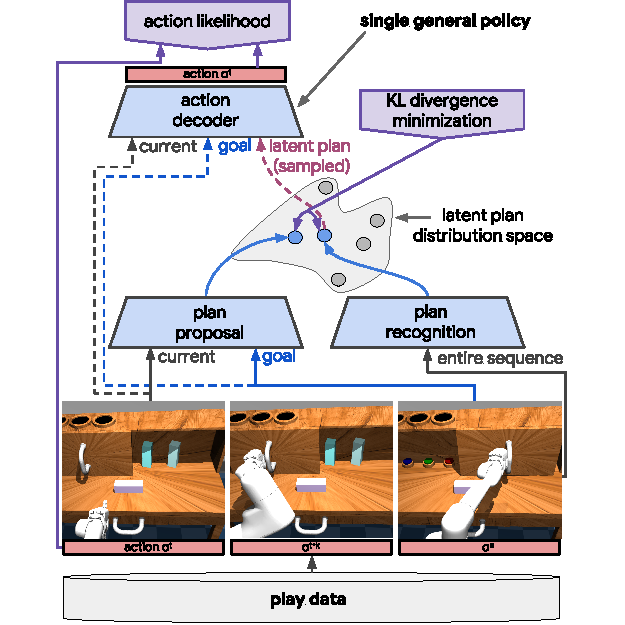
\includegraphics[height= 0.5\linewidth]{images/lmp_teaser5.pdf}
    \caption{Architecture used for the Learning from play method}
    \label{fig:LearningFromPlay}
\end{figure}


This approach has several key advantages:
\begin{itemize}
\item It is cheap: Large amounts of play data can be collected quickly since it doesn't require scene staging, task segmenting, or resetting to an initial state.
\item It is general: It encompasses both functional and non-functional behavior, relaxing the need for a predefined task distribution.
\item It is rich: Play naturally involves repeated, varied behavior, leading to high coverage of the possible interaction space. Additionally, the data is unlabeled, multimodal, and suboptimal.
\end{itemize}

\subsection{Resources}
There are many excellent resources on imitation learning and reinforcement learning. Much 
of the content presented here is based on Sergey Levine’s ''CS 285: Lecture 2 – Imitation 
Learning`` and ''Lecture 20 – Inverse Reinforcement Learning`` 
\cite{CS285,CS285LevineYoutube}. Additional resources that helped deepen my understanding 
of feature matching include ''Stanford CS234 – Reinforcement Learning | Offline RL 1 | 
2024, Lecture 8`` \cite{CS234Stanford}, and ''Maximum Entropy Inverse RL and Adversarial 
Imitation Learning`` by Katerina Fragkiadaki \cite{DeepRLandControl}. Another valuable 
reference on adversarial approaches is ''Deep RL Bootcamp – Lecture 10B: Inverse 
Reinforcement Learning`` \cite{DeepRlBootcamp}.

%    \item \href{https://www.youtube.com/watch?v=kGc8jOy5_zY}{CS 182: Lecture 14: Imitation Learning}
